\chapter{ÁP DỤNG CÁC GIẢI PHÁP ĐỀ XUẤT TRÊN DỮ LIỆU THỰC}
Sau khi đề xuất các kịch bản và các giải pháp lý thuyết ở chương trước, trong nội dung chương này nhóm tác giả tập trung xây dựng ứng dụng cụ thể để giải quyết bài toán hạn chế sự lan truyền của thông tin sai lệch trên mạng xã hội tại Việt Nam.

Nhóm tác giả đề xuất một giải pháp tổng thể bao gồm bốn bước
\begin{itemize}
	\item Bước đầu tiên: Thu thập dữ liệu. Trong bước này sau khi tiến hành khảo sát nguồn phát tán thông tin sai lệch, nhóm tác giả tiến hành xây dựng công cụ thu thập dữ liệu từ mạng xã hội Facebook xung quanh các nguồn phát tán trên.
	\item Bước thứ hai: Mô hình hóa dữ liệu. Dựa trên dữ liệu thu được, nhóm tác giả tiến hành mô hình hóa dữ liệu thu được dưới dạng đồ thị, thể hiện quá trình phát tán thông tin bằng hai mô hình tương ứng với hai kịch bản đã đề xuất ở chương trước.
	\item Bước thứ ba: Áp dụng hai kịch bản ngăn chặn và hai giải pháp tương ứng đã trình bày trong chương 3 đối với dữ liệu đã thu thập và đã được mô hình hóa.
	\item Bước cuối cùng: Ánh xạ người dùng thực. Bước này tiến hành ánh xạ ngược tập đỉnh thu được trong bước 3 nhằm thu được danh sách người dùng có vai trò quan trọng trong việc lan truyền thông tin sai lệch đối với 2 kịch bản ngăn chặn đã đề xuất.
\end{itemize}

Hình \ref{TongTheGiaiPhap} mô tả tổng thể giải pháp nhóm tác giả đề xuất
\begin{center}
	\begin{figure}[!htp]
		\begin{center}
			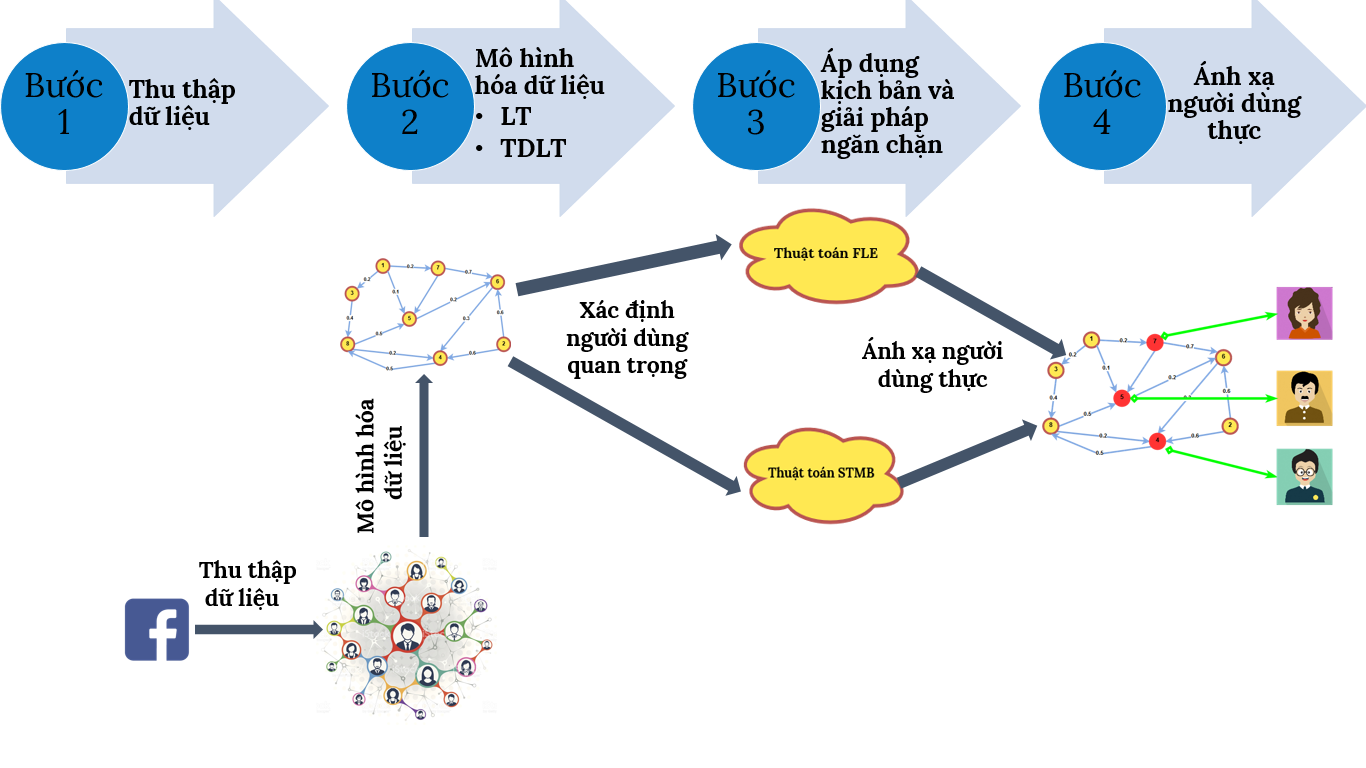
\includegraphics [scale=.3]{picture/TongTheGiaiPhap}
		\end{center}
		\caption{Tổng thể giải pháp}
		\label{TongTheGiaiPhap}
	\end{figure}
\end{center}

\section{Thu thập dữ liệu}

\subsection{Xác định nguồn phát tán thông tin sai lệch} \label{4.1.1}
Thông tin sai lệch phán tán trên mạng xã hội xuất phát từ các nguồn phát tán với tốc độ nhanh, quy mô rộng lớn. Đã có nhiều nghiên cứu đưa ra nhằm xác định các nguồn phát tán này, tuy nhiên hiệu quả và độ chính xác vẫn còn nhiều hạn chế. Trong thực tế, các nguồn phát tán thông tin sai lệch, các thông tin chống đối và xuyên tạc chính sách, đường lối của Đảng, pháp luật của Nhà nước thường là các đối tượng chủ mưu, cầm đầu, nắm vai trò quan trọng trong các tổ chức phản động. Đây là những đối tượng cơ hội chính trị, đối tượng bất mãn, đối tượng bảo thủ, ngoan cố và rất khó để thuyết phục các đối tượng đó gỡ bỏ các bài đăng, thông tin sai lệch trên mạng xã hội.

Trong nghiên cứu này, nhóm tác giả đã dùng phương pháp khảo sát, điều tra, theo dõi, nghiên cứu tài liệu để tìm ra những đối tượng có tính chất trên. Bằng các biện pháp này nhóm tác giả đã thu thập được nguồn phát tán thông tin sai lệch bao gồm 6 người dùng:

\begin {itemize}
\item https://www.facebook.com/gioan.namphong: Linh mục giáo sứ Thái Hà Nguyễn Nam Phong, một nhân vật khá nổi tiếng trong làng chống chính quyền trong nước và thường xuyên ra nước ngoài để "liên lạc" với tổ chức khủng bố Việt Tân.

\item https://www.facebook.com/minhnhat.paultran: Paul Trần Minh Nhật là giáo dân thuộc xứ Ngọc Long, xã Công Thành, Yên Thành, Nghệ An, từng bị bắt và kết án 4 năm tù về tội “hoạt động nhằm lật đổ chính quyền nhân dân”. Hiện tại, Minh Nhật đang là cộng tác viên của trang “Tin mừng cho người nghèo”, mang danh nghĩa rao giảng tin mừng của Chúa, nhưng lại nhuốm màu sắc chính trị, luôn ủng hộ các đối tượng vi phạm pháp luật.

\item https://www.facebook.com/ThaiDung2016: Gioan Thái Văn Dung là sinh viên tốt nghiệp ngành tin học, đã tham gia quản lý cửa hàng Internet, Do hiểu biết được CNTT mà biết thêm về xã hội, tích cực truyền bá thông tin, hoạt động mạng, tham gia biểu tình chống TQ xâm lược.

\item https://www.facebook.com/pham.doan.trang: Nhà báo Phạm Đoan Trang, từng công tác tại Báo Pháp Luật thành phố Hồ Chí Minh. Tác giả của cuốn sách “Chính trị Bình Dân” có những nội dung nhạy cảm, mang tính chất kích động, chống phá chính quyền, Đảng và Nhà Nước.

\item https://www.facebook.com/jbnguyenhuuvinh: Anh Ba Sàm, tên thật là Nguyễn Hữu Vinh là một blogger, từng là công an và đảng viên Đảng Cộng sản Việt Nam, từng công tác ở Ủy ban Việt kiều Trung ương. Ông bị Chính phủ CHXHCN Việt Nam bắt giữ và bị cáo buộc và phạt tù 5 năm do có hành vi đăng tải các bài viết trên mạng Internet vi phạm Điều 258 Bộ Luật Hình sự năm 2015 sửa đổi bổ sung năm 2017 về Tội lợi dụng các quyền tự do dân chủ xâm phạm lợi ích của Nhà nước, quyền, lợi ích hợp pháp của tổ chức, công dân.

\item https://www.facebook.com/profile.php?id=100015485029386: Nguyễn Trọng đang sinh sống tại California, Hoa Kỳ. Lợi dụng quyền tự do dân chủ, thường xuyên có những bài viết xuyên tạc, chống phá đường lối chính sác của Đảng, pháp luật của Nhà nước.
\end {itemize}

\subsection{Xây dựng công cụ thu thập dữ liệu trên mạng xã hội Facebook}

Dưới những điều kiện khác nhau, như tiềm lực tài chính, khả năng thuyết phục, phạm vi lan truyền thông tin khác nhau, cùng với đó là các mục tiêu khác nhau, có thể kể đến ảnh hưởng lan truyền của thông tin sai lệch, tỉ lệ người dùng nhiễm thông tin sai lệch và với các mô hình lan truyền thông tin khác nhau. Nhóm tác giả đã tiến hành xây dựng công cụ thu thập dữ liệu trực tiếp từ mạng xã hội Facebook, với phạm vi xung quanh các đối tượng chống đối, đối tượng cầm đầu thu được trong bước khảo sát trên.

Facebook cho phép các nhà phát triển (Developers) có thể lấy được thông tin dữ liệu, tuy nhiên điều đó phải được sự cho phép của người dùng thông qua các mã truy cập Access Token (Access Token là một đoạn mã do MXH sinh ra ngẫu nhiên khi người dùng đồng ý cho ứng dụng thứ 3 thực hiện các thao tác đối với tài khoản của người dùng). Điều này là một vấn đề khó khăn khi chúng ta cần khảo sát, lấy thông tin đối với một số lượng lớn người dùng nhằm xây dựng được đồ thị quan hệ giữa các người dùng trên MXH.

Một vấn đề khác là Facebook ngày càng thắt chặt các chính sách bảo mật đối với dữ liệu cá nhân của người sử dụng, trong đó bao gồm cả kiểm soát việc theo dõi thông tin cá nhân của người dùng bởi các người dùng khác. Facebook giới hạn thời gian, quyền truy cập, theo dõi đối với từng tài khoản Facebook, rộng hơn là từng địa chỉ IP trong việc truy cập thông tin cá nhân của người dùng khác.

Nhằm giải quyết vấn đề trên, nhóm tác giả đề xuất một hướng tiếp cận mới là sử dụng công cụ kiểm thử phần mềm tự động mã nguồn mở Selenium cho việc kiểm thử ứng dụng Web. Cụ thể ở đây nhóm tác giả thư viện mã nguồn mở của Selenium trên ngôn ngữ Python, kiểm thử tự động với trình duyện Chromnium.

	\subsubsection{Tổng quan về công cụ kiểm thử Selenium}
Selenium là một công cụ kiểm thử phần mềm tự động, được phát triển bởi ThoughtWorks từ năm 2004 với tên ban đầu là JavaScriptTestRunner. Đến năm 2007, tác giả Jason Huggins rời ThoughtWorks và gia nhập Selenium Team, một phần của Google và phát triển thành Selenium như hiện nay.

Selenium cung cấp công cụ phát lại (Playback) cho việc tạo ra các bài kiểm thử mà không cần phải học một ngôn ngữ kịch bản khác (Selenium IDE). Nó cũng cung cấp một ngôn ngữ thử nghiệm tên miền cụ thể (Selenese) để tạo ra các bài kiểm thử bằng một số ngôn ngữ lập trình phổ biến bao gồm C\#, Groovy, Java, Perl, Python, PHP, Ruby, Scala. Các thử nghiệm sau đó có thể chạy trên hầu hết các trình duyệt Web hiện đại. Selenium triển khai trên các nền tảng Windows, Linux và cả MacOS. Selenium là phần mềm mã nguồn mỡ, được phát hành theo giấy phép Apache 2.0.

Selenium bao gồm một số thành phần với mỗi thành phần tham gia vào một vai trò cụ thể trong việc hỗ trợ phát triển tự động kiểm tra ứng dụng Web, bao gồm: IDE Selenium, API Client Selenium, Selenium WebDriver, Selenium Remote Control và Selenium Grid. Trong nội dung đề tài nghiên cứu, nhóm tác giả sử dụng hai thành phần chính là API Client Selenium và Selenium WebDriver.

\begin{itemize}
	\item API Client Selenium
	Để thay thế cho các bài kiểm tra viết bằng Selen, các bài kiểm tra cũng có thể được viết bằng nhiều ngôn ngữ lập trình khác nhau. Những thử nghiệm này sau đó giao tiếp với Selenium bằng cách gọi các phương thức trong API ứng dụng khách Selenium. Selenium hiện cung cấp các API ứng dụng khách cho Java , C\#, Ruby , JavaScript và Python. Với Selenium 2, một API ứng dụng khách mới đã được giới thiệu (với WebDriver là thành phần trung tâm của nó). Tuy nhiên, API cũ (sử dụng lớp Selenium) vẫn được hỗ trợ.
	
	\item Selenium WebDriver
	Selenium WebDriver là sự kế thừa của Selenium RC. Selenium WebDriver chấp nhận các lệnh (được gửi bằng Selenese hoặc thông qua API ứng dụng khách) và gửi chúng tới trình duyệt. Điều này được thực hiện thông qua trình điều khiển trình duyệt cụ thể cho trình duyệt, trình điều khiển sẽ gửi lệnh tới trình duyệt và truy xuất kết quả. Selenium WebDriver không cần một máy chủ đặc biệt để thực hiện các thử nghiệm. Thay vào đó, WebDriver trực tiếp khởi động một cá thể trình duyệt và điều khiển nó. Tuy nhiên, Selenium Grid có thể được sử dụng với WebDriver để thực hiện các kiểm tra trên các hệ thống từ xa. Nếu có thể, WebDriver sử dụng chức năng cấp hệ điều hành gốc hơn là các lệnh JavaScript dựa trên trình duyệt để điều khiển trình duyệt. Điều này bỏ qua các vấn đề với sự khác biệt tinh tế giữa lệnh gốc và JavaScript, bao gồm cả các hạn chế bảo mật.
	
\end{itemize}	
	
	\subsubsection{Quá trình thu thập dữ liệu}

Các bước cụ thể của giai đoạn thu thập dữ liệu trên MXH Facebook được mô tả cụ thể như sau:
\begin {itemize}
\item Đầu tiên, nhóm tác giả tạo một tài khoản Facebook rồi sử dụng Công cụ kiểm thử tự động Selenium để tự động đăng nhập vào tài khoản Facebook đó.

\item Bằng các truy vấn đặc biệt, nhóm tác giả lấy được ID (Identity Number) của tài khoản trên.

\item Thông qua phương pháp giám sát và điều tra, thông qua những tin tức, vụ việc trong thời gian gần đây. Nhóm tác giả khảo sát dữ liệu với tập nguồn ban đầu bao gồm 6 tài khoản Facebook đã trình bày ở phần \ref{4.1.1}

\item Tiếp theo, nhóm tác giả tự động trup cập vào trang web có địa chỉ www.facebook.com/{ID}/friends hoặc www.facebook.com/{name}/friends là trang bạn bè của những người dùng đó.

\item Theo thuật toán sắp xếp của Facebook, những người dùng có liên quan nhất và hay tương tác nhất với người dùng đang theo dõi sẽ hiện ra đầu tiên trong trang bạn bè nói trên. Nhóm tác giả sử dụng thư viện BeautifulSoup để lấy mã HTML của trang này, tìm và lấy các đường dẫn chứa địa chỉ Facebook bạn bè của người dùng đang theo dõi, lấy ID của họ.

\item Nhóm tác giả thu thập theo phương pháp loang theo chiều rộng: Bắt đầu từ ID Facebook của 6 đối tượng kể trên, từ đó tìm tiếp thông tin về khoảng 20 người bạn xuất hiện đầu tiên trên trang Facebook bạn bè của mỗi người dùng đó. Với mỗi người dùng thu thập được, nhóm tác giả lại tiếp tục tiến hành thu thập như trên, và cứ tiếp tục tìm kiếm đến khi thu thập đủ số lượng người dùng cần thiết.
\end {itemize}		
Cách làm này có ưu điểm là những người dùng thu thập được có nhiều mối liên hệ với nhau, đồ thị MXH thu thập được có nhiều liên kết, mang lại sự trực quan hơn cho cấu trúc đồ thị mạng. Ngoài ra còn có quá trình tiền xử lý, bước này sẽ hạn chế, loại bỏ được những đỉnh cô lập, hay những đỉnh khai thác được ít thông tin (Không công khai danh sách bạn bè).

Bên cạnh những ưu điểm trên, thì cách làm này cũng có nhược điểm là không khai thác được hết thông tin của người dùng, bởi nhiều người dùng không để chế độ công khai bạn bè. Trong thực tế sẽ để lọt nhiều đối tượng nguy hiểm, ẩn chứa nhiều nguy cơ tiềm tàng.

\section{Mô hình hóa dữ liệu thu được}
Ở bước này, từ những dữ liệu thu thập được về danh sách ID người dùng, mối quan hệ bạn bè giữa họ. Nhóm tác giả tiền xử lý, đánh số lại các đỉnh, xây dựng đồ thị mô tả MXH với các đỉnh đại diện cho các người dùng, các cạnh biểu diễn mối quan hệ bạn bè giữa những người đó. Kết quả đầu ra của thuật toán thu thập thông tin trên MXH Facebook và quá trình chuẩn hóa, xử lý bao gồm 2 file dữ liệu:
\begin {itemize}
\item ID.txt chứa ánh xạ từ ID của người dùng sang chỉ số đỉnh được đánh số lại. Qua quá trình thu thập dữ liệu, chuẩn hóa, nhóm tác giả thu được 542 ID người dùng, được đánh số lại từ 0 – 541, xem bảng \ref{bang4_1}		
\begin{table} [!htp]
	\centering 
	\begin{tabular}{|c|c|}
		\hline 
		0 & 100003708850657 \\ 
		\hline 
		1 & 100009945675640 \\ 
		\hline 
		2 & 100010197936720 \\ 
		\hline 
		3 & 641613321 \\ 
		\hline 
		4 & 100002541019308 \\ 
		\hline 
		5 & 100015485029386 \\ 
		\hline 
		6 & 100004745583805 \\ 
		\hline 
		... & ... \\ 
		\hline 
		539 & 100004236103486 \\ 
		\hline 
		540 & 100004142778267 \\ 
		\hline 
		541 & 100006259445960 \\ 
		\hline 
	\end{tabular} 
	\caption{Ánh xạ ID người dùng sang chỉ số được đánh số - ID.txt}
	\label{bang4_1}
\end{table}
\item Network.txt chứa mô tả cụ thể của đồ thị MXH đã thu được. File dữ liệu gồm nhiều dòng, mỗi dòng chứa 2 số là chỉ số của 2 người dùng có quan hệ với nhau. Mô tả cụ thể được thể hiện trên bảng \ref{bang4_2}

\begin{table} [!htp]
	\centering
	\begin{tabular}{|c|c|}
		\hline 
		0 & 7 \\ 
		\hline 
		0 & 8 \\ 
		\hline 
		0 & 9 \\ 
		\hline 
		0 & 4 \\ 
		\hline 
		0 & 10 \\ 
		\hline
		0 & 11 \\ 
		\hline
		0 & 12 \\ 
		\hline  
		... & ... \\ 
		\hline 
		99 & 399 \\ 
		\hline 
		99 & 495 \\ 
		\hline 
		99 & 400 \\ 
		\hline 
		99 & 437 \\ 
		\hline 
		99 & 498 \\ 
		\hline 
	\end{tabular}
	\caption{Mô tả cụ thể của đồ thị MXH thu được - Network.txt}
	\label{bang4_2} 
\end{table}

Từ dữ liệu thu được, nhóm tác giả mô phỏng lại và thu được tổng quan về cấu trúc mạng như trên hình \ref{refhinh4_2} :

\begin{center}
	\begin{figure}[htp]
		\begin{center}
			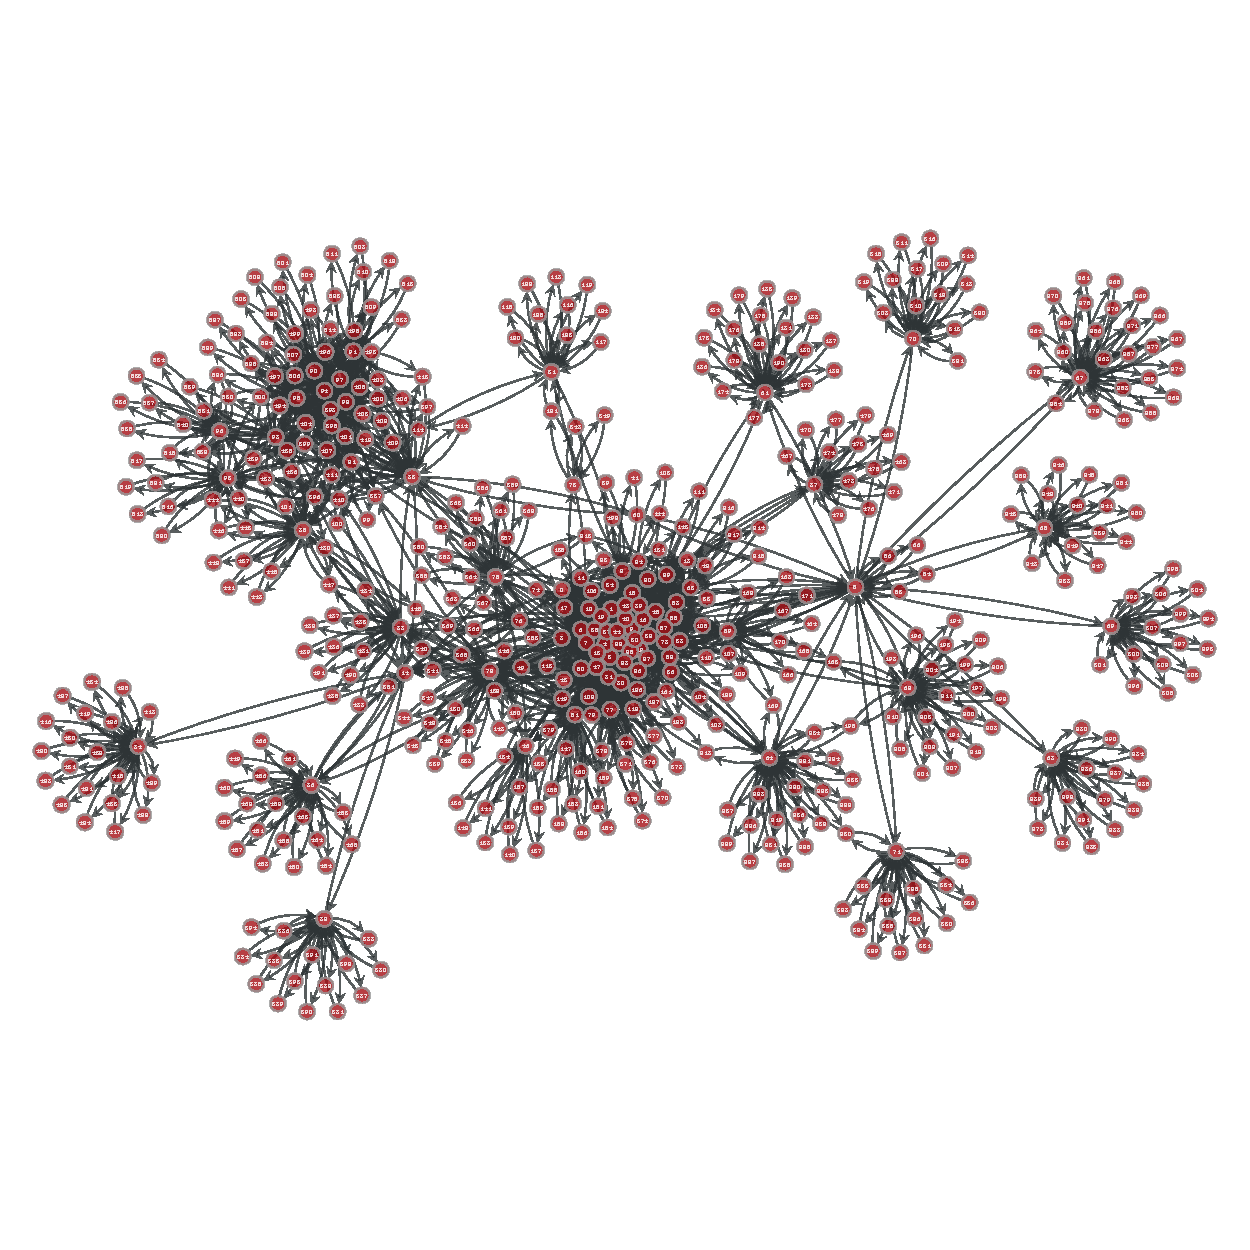
\includegraphics [scale=.6]{picture/Net}
		\end{center}
		\caption{Mô phỏng cấu trúc toàn mạng dữ liệu thu được}
		\label{refhinh4_2}
	\end{figure}
\end{center}
\end {itemize}

Tiếp theo, ứng với mỗi kịch bản ngăn chặn, mô hình phát tán thông tin tương ứng, nhóm tác giả tiến hành thiết lập trọng số đại diện cho mức độ tương tác giữa các người dùng với nhau, chuẩn hóa dữ liệu tương ứng với đầu vào yêu cầu của bài toán. Kết quả thu được như sau:

\begin{itemize}
	\item Đối với kịch bản FLE: Đầu vào là tệp tin input.inp chứa mô tả của đồ thị mạng xã hội, tập đỉnh nguồn phát tán thông tin sai lệch, số đỉnh cần xóa.
	File dữ liệu gồm nhiều dòng. 
	\begin{enumerate}
		\item Dòng đầu tiên chứa hai số nguyên dương cách nhau bởi một dấu cách $n m$. Trong đó $n$ là số đỉnh, $m$ là số cạnh của đồ thị.
		\item $m$ dòng tiếp theo, mỗi dòng chứa 3 số là chỉ số của 2 đỉnh có cạnh nối với nhau và trọng số cạnh tương ứng.
		\item Dòng tiếp theo là số nguyên $k$, số lượng đỉnh nguồn phát tán thông tin, cụ thể $k = 6$.
		\item $k$ dòng tiếp theo, mỗi dòng chứa một số nguyên dương là chỉ số đỉnh là nguồn phát tán thông tin của đồ thị, ở đây các đỉnh nguồn nhóm tác giả đánh số từ 1-6.
		\item Dòng cuối cùng là số nguyên đại diện số lượng đỉnh cần xóa.
	\end{enumerate}
	Mô tả cụ thể được thể hiện trên bảng \ref{bang4_3}
	
	\begin{table} [!htp]
		\centering
		\begin{tabular}{|c|c|c|}
			\hline 
			542 & 2336 & \\ 
			\hline 
			1 & 3 & 0.040\\ 
			\hline 
			1 & 5 & 0.030\\ 
			\hline 
			... & ... & ...\\ 
			\hline 
			542 & 100 & 0.062\\
			\hline
			6 & & \\
			\hline
			1 & & \\
			\hline
			2 & & \\
			\hline
			3 & & \\
			\hline
			4 & & \\
			\hline
			5 & & \\
			\hline
			6 & & \\
			\hline
			10 & & \\
			\hline 
		\end{tabular}
		\caption{Dữ liệu đầu vào ứng với giải pháp FLE - input.txt}
		\label{bang4_3} 
	\end{table}
	
	\item Đối với kịch bản STMB: Đầu vào bao gồm 2 tệp tin
	\begin{enumerate}
		\item Tệp tin TestFacebook.txt chứa mô tả đồ thị mạng xã hội. Tệp tin gồm nhiều dòng, mỗi dòng chứa 3 số là chỉ số của 2 đỉnh có cạnh nối với nhau và trọng số cạnh tương ứng.
		Mô tả cụ thể được thể hiện trên bảng \ref{bang4_4}
		\begin{table} [!htp]
			\centering
			\begin{tabular}{|c|c|c|}
				\hline 
				1 & 3 & 0.040\\ 
				\hline 
				1 & 5 & 0.030\\ 
				\hline 
				1 & 8 & 0.030\\ 
				\hline 
				1 & 9 & 0.025\\ 
				\hline 
				... & ... & ...\\ 
				539 & 98 & 0.062\\
				\hline 
				540 & 99 & 0.048\\
				\hline 
				541 & 100 & 0.062\\
				\hline 
				542 & 100 & 0.062\\		
				\hline 
			\end{tabular}
			\caption{Dữ liệu đầu vào ứng với giải pháp STMB - TestFacebook.txt}
			\label{bang4_4} 
		\end{table}
	
		\item Tệp tin TestSourceFacebook.txt chứa tập chỉ số các đỉnh nguồn phát tán thông tin. Tệp tin gồm 6 dòng, mô tả cụ thể thể hiện trên bảng \ref{bang4_5}
		\begin{table} [!htp]
			\centering
			\begin{tabular}{|c|}
				\hline
				1\\	
				\hline 
				2\\	
				\hline 
				3\\	
				\hline 
				4\\	
				\hline 
				5\\	
				\hline 
				6\\	
				\hline 
			\end{tabular}
			\caption{Dữ liệu đầu vào ứng với giải pháp STMB - TestSourceFacebook.txt}
			\label{bang4_5} 
		\end{table}
	\end{enumerate}
	\end{itemize}
	
\section{Áp dụng kịch bản và giải pháp ngăn chặn}

Trong bước này, nhóm tác giả tiến hành áp dụng hai giải pháp ngăn chặn tương ứng với hai kịch bản đã đề xuất đối với các dữ liệu thực đã thu thập từ mạng xã hội Facebook và đã được mô hình hóa. Kết quả thu được đối với từng giải pháp như sau:

\begin{itemize}
	\item Áp dụng giải pháp FLE đối với kịch bản LSE. Kết quả được lưu lại trong tệp tin Output.txt, được mô tả cụ thể trên bảng \ref{bang4_6}.
	\begin{table} [!htp]
		\centering
		\begin{tabular}{|c|}
			\hline
			8 -> 100002788524244\\
			\hline
			15 -> 634032152\\
			\hline
			18 -> 100000315904157\\
			\hline
			19 -> 1849592060\\
			\hline
			22 -> 100004460193964\\
			\hline
			30 -> 100003888766757\\
			\hline
			39 -> 100000757109103\\
			\hline
			115 -> 100001730194864\\
			\hline
			338 -> 100005228346422\\
			\hline
			397 -> 100003276218628\\
			\hline
			Saved = 150\\
			\hline 
		\end{tabular}
		\caption{Kết quả thực hiện giải pháp FLE với dữ liệu thu thập - Output.txt}
		\label{bang4_6} 
	\end{table}
	
	So sánh kết quả thực nghiệm này đối với các thuật toán MaxDegree và Random về mặt số lượng đỉnh được cứu, thu được kết quả như hình \ref{fig:FLE_FB}:
	
	\begin{center}
		\begin{figure}[htp]
			\begin{center}
				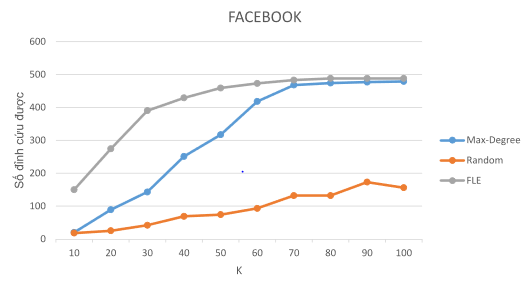
\includegraphics [scale = 1.2]{picture/FLE/FB_res}
			\end{center}
			\caption{So sánh chất lượng lời giải của các thuật toán với dữ liệu Facebook}
			\label{fig:FLE_FB}
		\end{figure}
	\end{center}	
	Trong hình \ref{fig:FLE_FB}, ta có thể thấy rằng FLE, với cùng một ngưỡng số đỉnh tối đa cứu được chặn là $k$, luôn đạt được kết quả tốt hơn so với hai thuật toán còn lại. Đặc biệt, với $k>=80$, thuật toán FLE chỉ ra được phương pháp chặn bắt để số đỉnh cứu được là tối đa, điều mà hai thuật toán Random và MaxDegree dù với $k=100$ cũng không thể làm được.
	
	Vì số đỉnh của đồ thị thu được là khá nhiều cho việc mô tả chỉ tiết nên chúng tôi lựa chọn một phần của đồ thị để mô phỏng, mà cụ thể là phần trung tâm của đồ thị (phần tập trung nguồn phát tán thông tin sai lệch). Sử dụng công cụ graph\_tool\footnote{https://graph-tool.skewed.de/}, chúng tôi cỏ thể mô tả lại một phần mạng dữ liệu được sử dụng như hình \ref{fig:FLE_MP}:
	
	\begin{center}
		\begin{figure}[htp]
			\begin{center}
				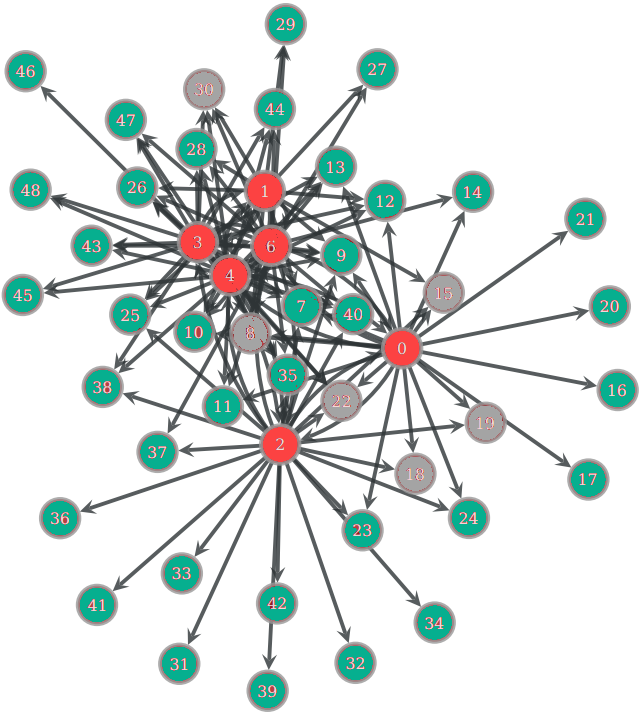
\includegraphics[scale=.7]{picture/PartMH}
			\end{center}
			\caption{Kết quả mô phỏng với dữ liệu thu thập được trên Facebook của thuật toán FLE}
			\label{fig:FLE_MP}
		\end{figure}
	\end{center}
	
	Các đỉnh được tô màu đỏ thể hiện nguồn phát tán thông tin sai lệch, các đỉnh được tô màu xám là tập đỉnh được lụa chọn để loại ra đồ thị theo kết quả thuật toán, các đỉnh còn lại sẽ được tô màu xanh.


	\item Áp dụng giải pháp STMB đối với kịch bản TMB. Kết quả được lưu lại trong các tệp tin có cấu trúc tên là Seed\_STMB\_Facebook\_x$\cdot$y$\cdot$txt chứa thông tin về các chỉ số đỉnh tìm được, mỗi đỉnh một dòng, trong đó $x$ là số lần lấy mẫu, $y$ là ngưỡng của bài toán đặt ra.
	Ngoài ra kết quả tổng hợp được lưu trong tệp tin Result.txt, được mô tả cụ thể trên bảng \ref{bang4_7}.
	
	\begin{table} [!htp]
		\centering
		\begin{tabular}{|c|}
			\hline
			|V| = 536\\
			\hline
			sigma comming : 74.84\\
			\hline
			Hmax = 12.841\\
			\hline
			Threshold = 3\\
			\hline
			Hmax = 12.841\\
			\hline
			Threshold = 6\\
			\hline
			Hmax = 12.841\\
			\hline
			Threshold = 9\\
			\hline
			...\\
			\hline
			Hmax = 28.288\\
			\hline
			Threshold = 24\\
			\hline
			Hmax = 28.288\\
			\hline
			Threshold = 27\\
			\hline
			Hmax = 32.827\\
			\hline
			Threshold = 30\\
			\hline 
		\end{tabular}
		\caption{Kết quả thực hiện giải pháp SMTB với dữ liệu thu thập - Result.txt}
		\label{bang4_7} 
	\end{table}
	So sánh kết quả thực nghiệm của các thuật toán STMB, Greedy, PageRank, High-Degree về mặt số lượng đỉnh tìm được thỏa mãn yêu cầu (càng ít đỉnh càng tốt), ta thu được hình \ref{realData_TMB}
	\begin{center}
		\begin{figure}[H]
			\begin{center}
				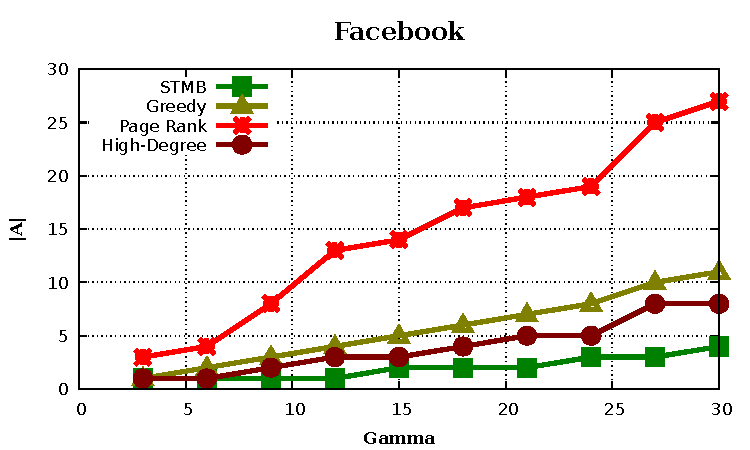
\includegraphics [scale=1]{picture/Facebook}
			\end{center}
			\caption{So sánh chất lượng lời giải của các thuật toán với dữ liệu thu thập được cho bài toán TMB}
			\label{realData_TMB}
		\end{figure}
	\end{center}

	Trong hình \ref{realData_TMB}, ta có thể thấy rằng số đỉnh tìm được để thỏa mãn yêu cầu của STMB luôn là nhỏ nhất trong 4 thuật toán. 
	
	Về mặt thời gian thực hiện, STMB cũng thể hiện tốc độ vượt trội của mình so với các thuật toán được đánh giá là thời gian thực thi thấp như Page Rank hay High-Degree. Do thời gian thực hiện của thuật toán Greedy với dữ liệu thu thập được trung bình hơn 400(s) lâu hơn rất nhiều so với các thuật toán khác nên chúng tôi không đưa ra trong hình \ref{timeface}.
	\begin{center}
		\begin{figure}[H]
			\begin{center}
				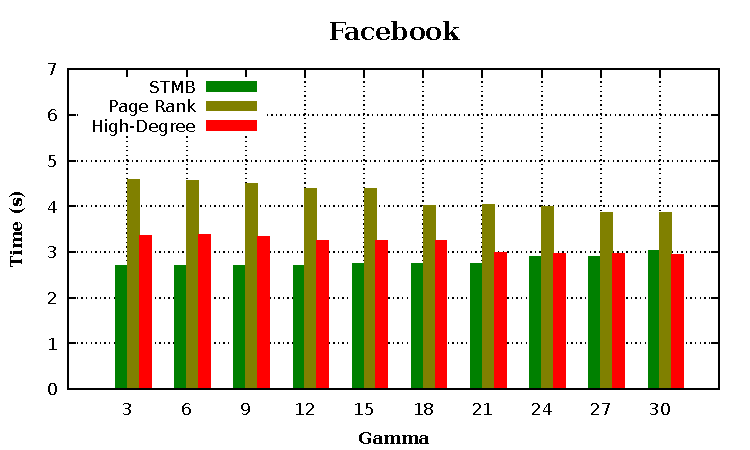
\includegraphics [scale=1]{picture/TimeFacebook}
			\end{center}
			\caption{So sánh thời gian thực hiện của các thuật toán với dữ liệu thu thập được cho bài toán TMB}
			\label{timeface}
		\end{figure}
	\end{center}
	
	Tiếp tục sử dụng công cụ graph\_tool chúng tôi mô phỏng lại phần trung tâm của đồ thị  và thu được kết quả như trong hình \ref{mophong}.
	
	\begin{center}
		\begin{figure}[H]
			\begin{center}
				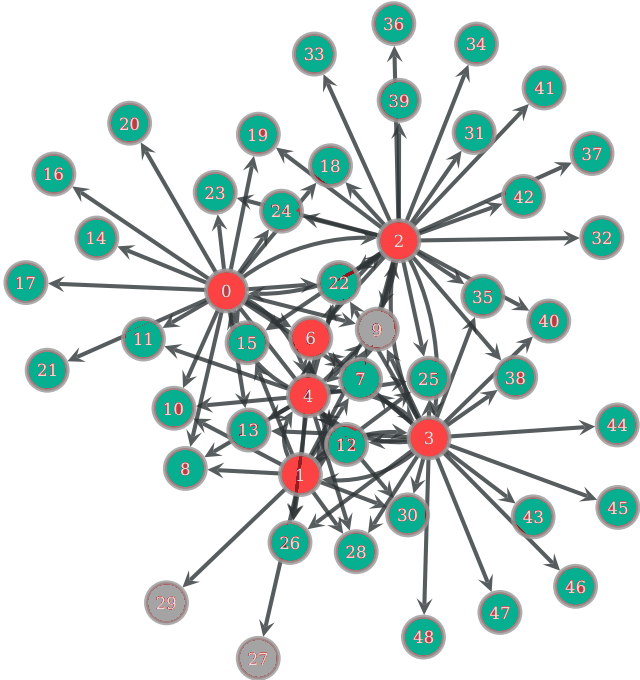
\includegraphics [scale=.7]{picture/PartPVQ}
			\end{center}
			\caption{Kết quả mô phỏng với dữ liệu thu thập được trong trường hợp $\gamma = 15$ của thuật toán STMB}
			\label{mophong}
		\end{figure}
	\end{center}
	
	Với các đỉnh được tô màu đỏ thể hiện nguồn phát tán thông tin sai lệch, các đỉnh được tô màu xám là tập đỉnh cần loại bỏ ra khỏi đồ thị, các đỉnh còn lại được tô màu xanh.
\end{itemize}
	

	
\section{Giải pháp Limiting the spread of epidemics within time constraint on online social network}

\subsection{Dữ liệu thu thập được}

Với dữ liệu thu thập được từ phần \ref{data}, chúng tôi chuẩn hóa dữ liệu theo mô hình T-DLT, sau đó thực nghiệm với các thuật toán MaxDegree, Random và FLE như được trình bày ở trên và thu được kết quả như hình \ref{fig:FLE_FB}:



\section{Giải pháp Targeted Misinformation Blocking (Xác định và ngăn chặn thông tin sai lệch trên mạng xã hội)}


\subsection{Dữ liệu thu thập được}	
Với dữ liệu thu được ở phần \ref{data} trong chương 4, chúng tôi chuẩn hóa dữ liệu theo mô hình LT, sau đó thực nghiệm với các thuật toán được nêu trong phần trước. Kết quả thu được như sau:



